% Essential Formatting

\documentclass[12pt]{article}
\usepackage{epsfig,amsmath,amsthm,amssymb, graphicx}
\usepackage[questions, answersheet]{urmathtest}[2001/05/12]
%\usepackage[answersheet]{urmathtest}[2001/05/12]
%\usepackage[answers]{urmathtest}[2001/05/12]


% For use with pdflatex
% \pdfpagewidth\paperwidth
% \pdfpageheight\paperheight

% Basic User Defs

\def\ds{\displaystyle}

\newcommand{\ansbox}[1]
{\work{
  \pos\hfill \framebox[#1][l]{ANSWER:\rule[-.3in]{0in}{.7in}}
}{}}

\newcommand{\ansrectangle}
{\work{
  \pos\hfill \framebox[6in][l]{ANSWER:\rule[-.3in]{0in}{.7in}}
}{}}


% Beginning of the Document

\begin{document}
\examtitle{LINEAR REGRESSION MODELS W4315}{HOMEWORK 1}{09/16/2009}
 \begin{center}
  Professor: Frank Wood
 \end{center}
%%\studentinfo
\instructions{
  %\textbf{Circle your Instructor's Name along with the Lecture Time:}



  \begin{itemize}
  \item
    \textbf{Please show all your work.
            You may use back pages if necessary.}
  %\item
   % \textbf{Please put your \underline{simplified}
   %         final answers in the spaces provided.}
  \end{itemize}
}
\finishfirstpage

% Problems Start Here % ----------------------------------------------------- %


\problem{20} { Let $Y_i = \beta_0 + \beta_1 X_i + \epsilon_i$ be a
linear regression model with distribution of error terms unspecified
(but with mean $E(\epsilon) = 0$ and variance $V(\epsilon_i) =
\sigma^2$ ($\sigma^2$ finite) known).  Show that $s^2 = MSE =
\frac{\sum(Y_i-\hat Y_i)^2}{n-2}$ is an unbiased estimator for
$\sigma^2$.  $\hat Y_i = b_0 + b_1 X_i$ where $b_0 = \bar Y - b_1
\bar X$ and $b_1 = \frac{\sum_i((X_i-\bar X)(Y_i - \bar
Y))}{\sum_i(X_i-\bar X)^2}$. } { \vfill
  \answer
}
{
First, let's denote the followings:\\
\begin{equation*}
\begin{array}{l}
\hat{e_i}=y_i-\hat{y_i}\\
S_{XX}=\displaystyle\sum_{i=1}^n (x_i-\bar{x})^2=\displaystyle\sum_{i=1}^n x_i^2-n\bar{x}^2\\
S_{YY}=\displaystyle\sum_{i=1}^n (y_i-\bar{y})^2=\displaystyle\sum_{i=1}^n y_i^2-n\bar{y}^2\\
S_{XY}=\displaystyle\sum_{i=1}^n (x_i-\bar{x})(y_i-\bar{y})=\displaystyle\sum_{i=1}^n (x_i-\bar{x})y_i
\end{array}
\end{equation*}
Consequently, $b_1=S_{XY}/S_{XX}$.

Now we set out to prove the following equation which essentially accomplishes the final result:\\
\[Var\hat{e_i}=E\hat{e_i}^2=(\frac{n-2}{n}+\frac{1}{S_{XX}}(\frac{1}{n}\displaystyle\sum_{j=1}^nx_j^2+x_i^2-2(x_i-\bar{x})^2-2x_i\bar{x}))\sigma^2\]
To prove the above display, realize that:\\
\begin{align*}
Var(\hat{e_i})&=Var(y_i-b_0-b_1x_i)\\
              &=Var((y_i-\beta_0-\beta_1x_i)-(b_0-\beta_0)-x_i(b_1-\beta_1))\\
              &=Var(y_i)+Var(b_0)+x_i^2Var(b_1)-2Cov(y_i,b_0)-2x_iCov(y_i,b_1)+2x_iCov(b_0,b_1)\\
\end{align*}
The last equation holds because the covariance between any random
variable and a constant is zero, and all the $y_i$'s are independent
entailing that the $Cov(y_i,y_j)=0,i\not=j$\\

Then we need to calculate each term of the above display
\begin{align*}
 Var(b_1)&=Var(\frac{S_{XY}}{S_{XX}})\\
             &=Var(\frac{\sum{(x_i-\bar{x})}y_i}{S_{XX}})\\
             &=\frac{1}{S_{XX}^2}\sum(x_i-\bar{x})^2Var(y_i)\\
             &=\frac{\sigma^2}{S_{XX}}\\
\end{align*}
And:\\
\begin{align*}
 Var(b_0)&=Var(\bar{y}-b_1\bar{x})\\
             &=Var(\sum{(\frac{1}{n}-\frac{(x_i-\bar{x})\bar{x}}{S_{XX}})y_i})\\
             &=\sum{(\frac{1}{n}-\frac{x_i-\bar{x}}{S_{XX}}\bar{x})^2}\sigma^2\\
             &=\sum{[\frac{1}{n^2}+\frac{(x_i-\bar{x})^2*\bar{x}^2}{S_{XX}^2}-\frac{2}{n}\frac{\bar{x}(x_i-\bar{x})}{S_{XX}}]}\sigma^2\\
             &=[\frac{1}{n}+\frac{\bar{x}^2}{S_{XX}}]\sigma^2\\
             &=\frac{\sum{x_i}^2}{n*S_{XX}}\sigma^2
\end{align*}
For the other terms in the decomposition of $Var(\hat{e_i})$, we
have:\\
\begin{align*}
 Cov(y_i,b_1)&=Cov(y_i,\frac{\sum(x_i-\bar{x})y_i}{S_{XX}})\\
                       &=\frac{x_i-\bar{x}}{S_{XX}}Var(y_i)\\
                       &=\frac{x_i-\bar{x}}{S_{XX}}\sigma^2
\end{align*}
and:\\
\begin{align*}
 Cov(y_i,b_0)&=Cov(y_i,\bar{y}-b_1\bar{x})\\
                       &=Cov(y_i,\frac{\sum{y_i}}{n}-\frac{\sum{(x_i-\bar{x})y_i}}{S_{XX}}\bar{x})\\
                       &=\frac{\sigma^2}{n}+\bar{x}\frac{x_i-\bar{x}}{S_{XX}}\sigma^2
\end{align*}
At last, we have:\\
\begin{align*}
 Cov(b_0,b_1)&=Cov(\bar{y}-b_1\bar{x},b_1)\\
                                 &=Cov(\frac{\sum{y_i}}{n}-\sum{\frac{(x_i-\bar{x})\bar{x}}{S_{XX}}}y_i,\sum{\frac{(x_i-\bar{x})y_i}{S_{XX}}})\\
                                 &=\displaystyle\sum_{i=i}^{n}(\frac{1}{n}-\frac{x_i-\bar{x}}{S_{XX}}\bar{x})\frac{x_i-\bar{x}}{S_{XX}}\sigma^2\\
                                 &=-\frac{\bar{x}}{S_{XX}}\sigma^2
\end{align*}
Then plug in all the parts back to the decomposition of
$Var(\hat{e_i})$, we have:\\
$Var(\hat{e_i})=(\frac{n-2}{n}+\frac{1}{S_{XX}}(\frac{1}{n}\displaystyle\sum_{j=1}^{n}{x_j}^2+x_i^2-2(x_i-\bar{x})^2-2x_i\bar{x}))\sigma^2$\\
\noindent Thus,\\
\begin{align*}
 E\hat{\sigma}^2&=\frac{1}{n-2}\displaystyle\sum_{i=1}^{n}E\hat{e_i}^2\\
                &=\frac{1}{n-2}\displaystyle\sum_{i=1}^{n}[\frac{n-2}{n}+\frac{1}{S_{XX}}(\frac{1}{n}\displaystyle\sum_{j=1}^{n}x_j^2+x_i^2-2(x_i-\bar{x})^2-2x_i\bar{x})]\sigma^2\\
                &=[1+\frac{1}{nS_{xx}}\{\displaystyle\sum_{j=1}^{n}x_j^2+\displaystyle\sum_{i=1}^{n}x_i^2-2S_{XX}-2\frac{1}{n}(\displaystyle\sum_{i=1}^{n}x_i)^2\}]\sigma^2\\
                &=(1+0)\sigma^2\\
                &=\sigma^2\\
\end{align*}
where the third equation holds because:
$\sum x_i\bar{x}=\frac{1}{n}(\sum{}{} x_i)^2$\\
and the second to last equation holds since
$\sum x_i^2-\frac{1}{n}(\sum{}{} x_i)^2=S_{XX}$\\
From the above equation, the result flows. \\
}

\problem{20} { Derive the maximimum likelihood estimators $\hat
\beta_0, \hat \beta_1,$ and $\hat \sigma^2$ for parameters $\beta_0,
\beta_1,$ and $\sigma^2$ for the normal linear regression model
(i.e.~$\epsilon_i \sim_{iid} N(0,\sigma^2)$). } { \vfill
  \answer
}
{
To figure the MLE of the parameters, we need to first write down
the likelihood function of the data, so under normal assumption, we
have the log-likelihood function as follows:\\
$logL(\beta_0,\beta_1,\sigma^2|x,y)=-\frac{n}{2}log(2\pi)-\frac{n}{2}log\sigma^2-\frac{\displaystyle\sum_{i=1}^{n}(y_i-\beta_0-\beta_1x_i)^2}{2\sigma^2}.$\\
For any fixed value of $\sigma^2$, $logL$ is maximized as a function
of $\beta_0$ and $\beta_1$, that minimize
\begin{eqnarray}
\displaystyle\sum_{i=1}^{n}(y_i-\beta_0-\beta_1x_i)^2
\end{eqnarray}
But to minimize this function is just to principle behind LSE, so
it's apparent that the MLE of $\beta_0$ and $\beta_1$ are the same
as their LSE's. Now, substituting in the log-likelihood, to find the
MLE of $\sigma^2$ we need to maximize\\
\[-\frac{n}{2}log(2\pi)-\frac{n}{2}log\sigma^2-\frac{\displaystyle\sum_{i=1}^{n}(y_i-b_0-b_1x_i)^2}{2\sigma^2}\]\\
This maximization problem is nothing but MLE of $\sigma^2$ in
ordinary normal sampling problems, which is easily given as\\
\[\hat{\sigma}^2=\frac{1}{n}\displaystyle\sum_{i=1}^{n}(y_i-b_0-b_1x_i)^2\]\\
If you are not familiar with the MLE in normal sampling setting, you
can take derivative with respect to $\sigma^2$ (N.B. not $\sigma$),
and then set the derivative to be zero. The solution of the equation
is just the MLE of $\sigma^2$.\\
}


\problem{20} {$X_1,X_2,X_3,\ldots,X_{100}$ are iid normal random 
variables with mean $\mu$ and variance $\sigma^2$, we want to estimate 
the mean $\mu$. Consider two estimators, $X_1$ and $\bar{X}=\frac{1}{100}\sum_{i=1}^{100}X_i$: \\
a. Show these two estimators are both unbiased. Also derive the
distribution of each estimator. Which estimator do you think is better? Why?\\
b. When $\mu=0$ and $\sigma^2=100$, generate $X_1,X_2,X_3,\ldots,X_{100}$. Calculate the estimate $\bar{X}$ and denote
it as $\hat{\mu}_1$. Repeat this 100 times and plot the density histogram of $\hat{\mu}_1,
\hat{\mu}_2,\hat{\mu}_3,\ldots,\hat{\mu}_{100}$. Overlay the probability density of $\bar{X}$ on the plot (see matlab function ``normpdf''). \\}
 { \vfill
  \answer
}
 {
 a. $X_1$ is unbiased is pretty obvious, for $\bar{X}$, using linearity of expectation, we have
  \[E(\bar{X})=E(\frac{1}{100}\sum_{i=1}^{100}X_i)=\frac{1}{100}\sum_{i=1}^{100}EX_i=\frac{1}{100}\sum_{i=1}^{100}\mu=\mu \]\\
   Apprantly, $X_1\sim N(\mu,\sigma^2)$. $\bar{X}$ is a linear combination of normal random variables, so it is still a normal random variable. Thanks to indepedence, its variance is given by 
   \[Var(\bar{X})=\frac{1}{100^2}Var(\sum_{i=1}^{100}X_i)=\frac{1}{100^2}\sum_{i=1}^{100}Var(X_i)=\frac{\sigma^2}{100}\]
  so $\bar{X}\sim N(\mu, \frac{1}{100}\sigma^2)$. Obviously, $\bar{X}$ is better since it has smaller variance.\\

 b.
 \begin{figure}[htbp]
  \centering
  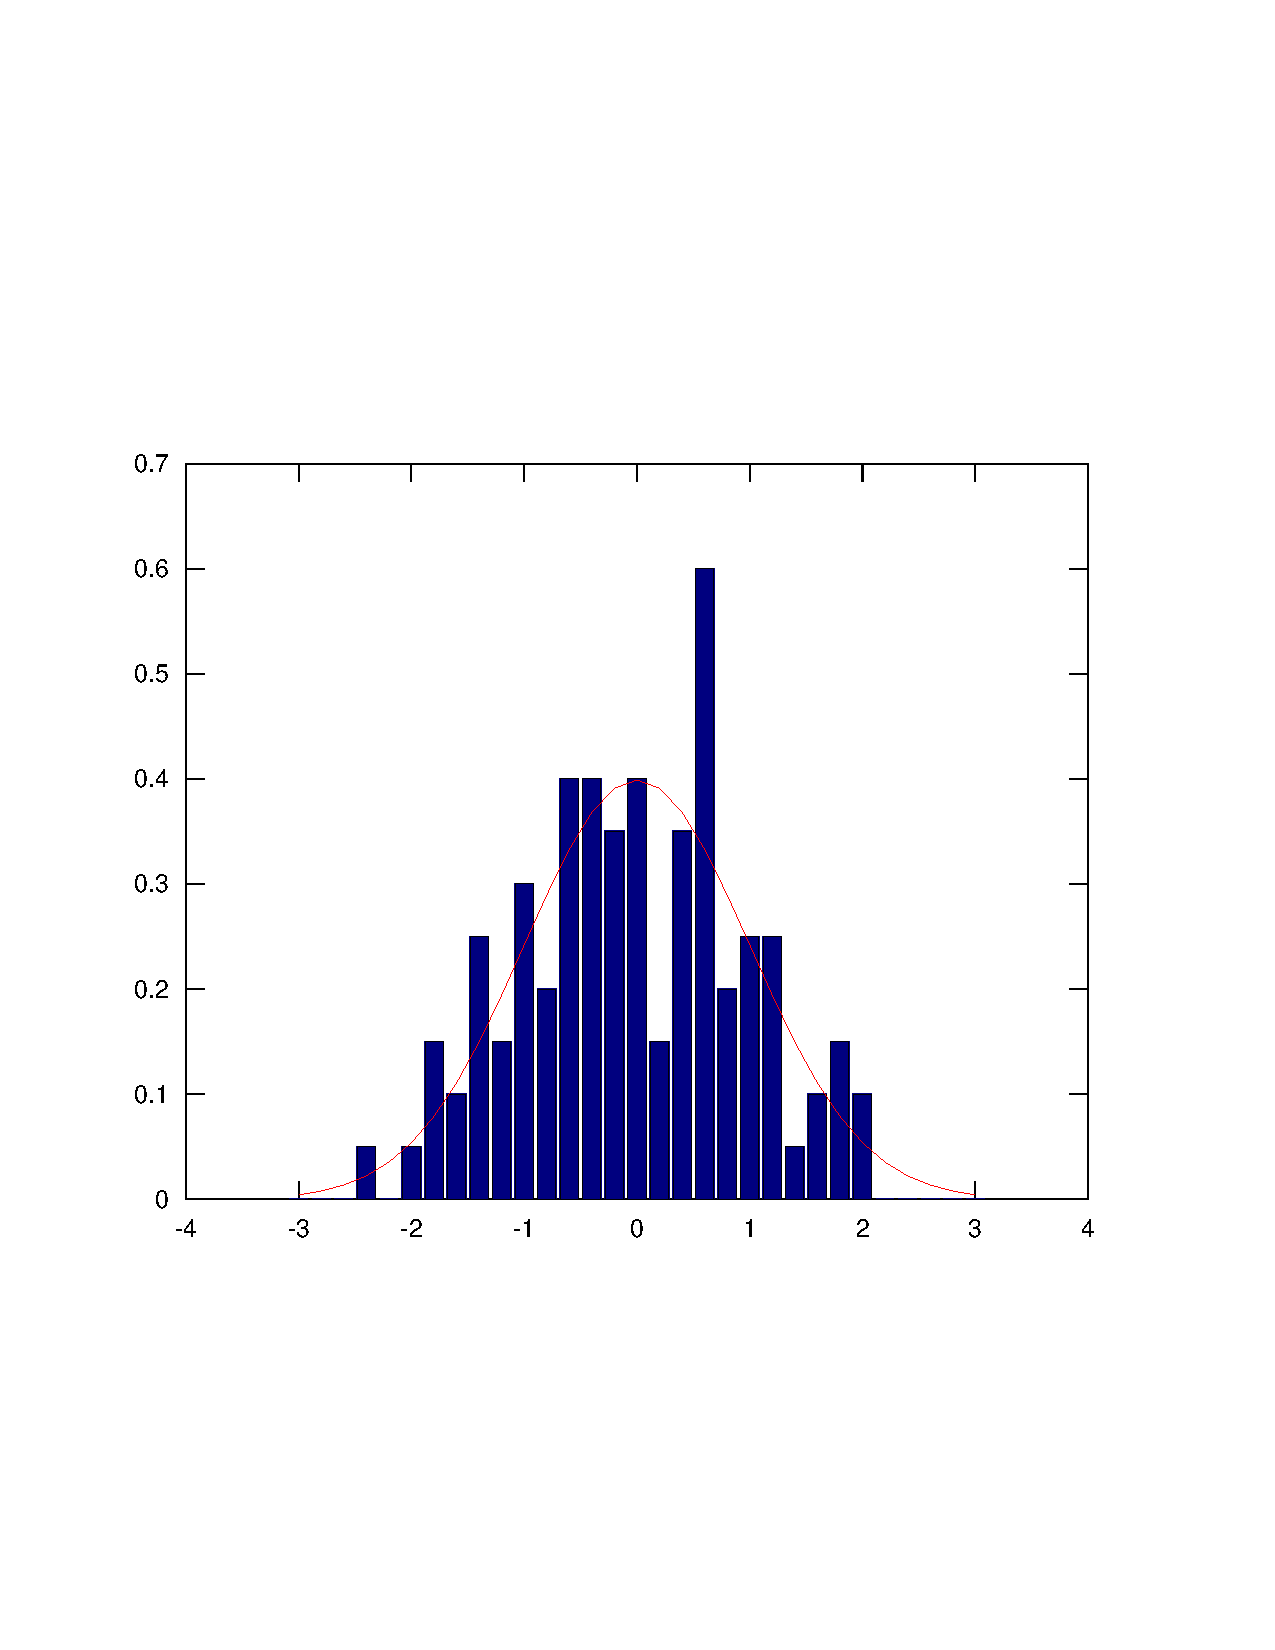
\includegraphics[width=8cm]{hist.pdf}
  \end{figure}

} 



\problem{40} { \textbf{Copier maintenance.}\footnote[1]{This is
problem 1.20 in ``Applied Linear Regression Models(4th edition)'' by
Kutner etc. )} The Tri-City Office Equipment Corporation sells an
imported copier on a franchise basis and performs preventive
maintenance and repair services on this copier. The data below have
been collected from 45 recent calls on users to perform routine
preventive number of minutes spent by the service person. Assume
that first-order regression model($Y_i=b_0+b_1 X_i+\epsilon_i$) is
appropriate.
\begin{table}[htdp]
\begin{center}
\begin{tabular}{rcrcrcrcrcrcrcrc}
\textbf{i:} &\textbf{1} &\textbf{2}& \textbf{3}&...&\textbf{43}&\textbf{44}&\textbf{45}\\
\hline \textbf{$X_i$} &2 &4 &3 &... &2 &4 &5\\
\textbf{$Y_i$} &20 &60 &46 &... &27 &61 &77
\end{tabular}
\end{center}
\end{table}\\

a. Obtain estimated regression function.\\
b. Plot the estimated regression function and the data. How well
does the estimated regression function fit the data?\\
c. interpret $b_0$ in your estimated regression function. Does $b_0$
provide any relevant information here? Explain.\\
d. Obtain a point estimate of the mean service time when $X=5$
copiers are serviced.\\
\indent~~~~Notice: You can get data for this problem on
www.mhhe.com/KutnerALRM4e. Use MATLAB, do not
use any other programming language. Only basic MATLAB operators are
allowed, do not use any built-in functions to do the regression, i.e.~the function ``regress'' cannot be used except, perhaps, to verify that your answer is correct before submitting your own implementation. \\}
 { \vfill
  \answer
} {
  a. $y = -0.58 + 15.04*x + \epsilon$; 

  b. Based on the graph, the model fit quite well.
\begin{figure}[htbp]
  \centering
  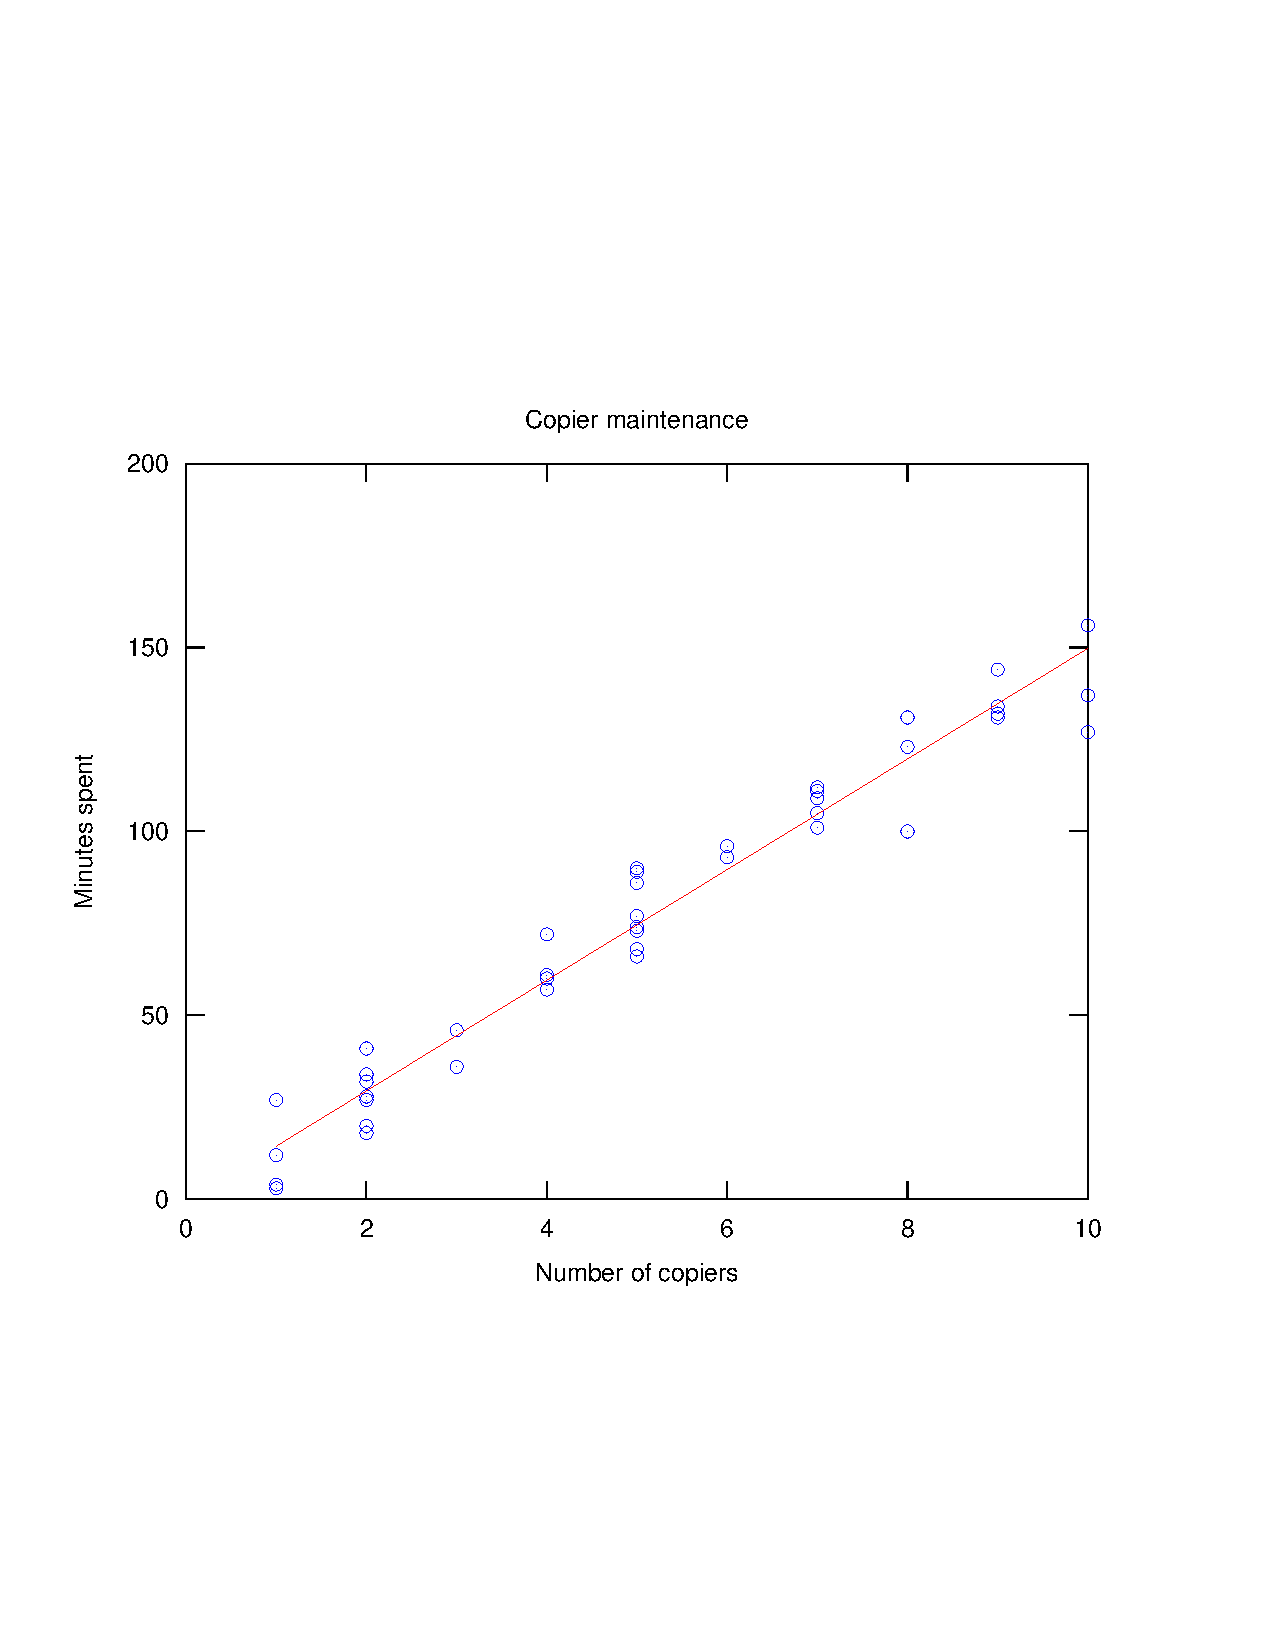
\includegraphics[width=8cm]{graph.pdf}
  \end{figure}
  
  c. $b_0=-0.58$ means number of minutes spent to servie 0 copier, which doesn't make any practical sense.

  d. $5*b_1+b_0=74.596$.
} 


% Problems End Here % ------------------------------------------------------- %

\problemsdone
\end{document}

% End of the Document
